\documentclass[11pt]{article}
\usepackage[margin=1in]{geometry}
\usepackage{tikz}
\usetikzlibrary{positioning, arrows.meta, calc}
\usepackage{amsmath}
\usepackage{amssymb}

\begin{document}

\begin{figure}[t]
\centering
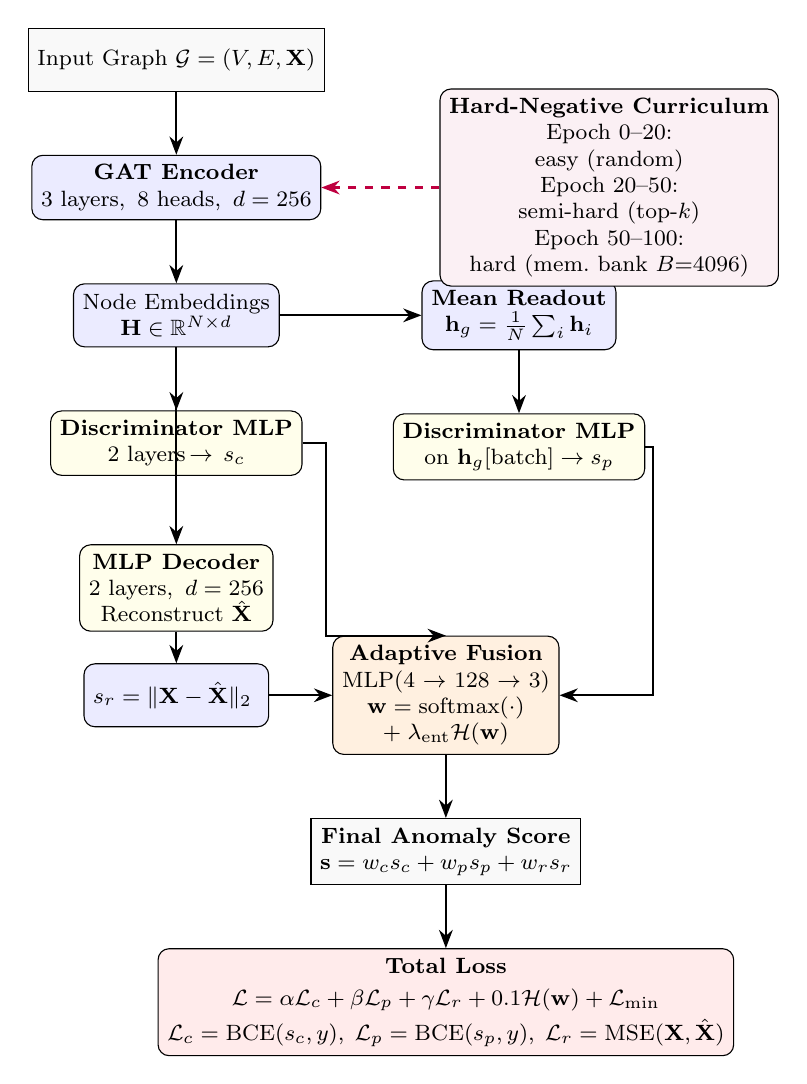
\begin{tikzpicture}[
    node distance=0.8cm and 1.8cm,
    block/.style={rectangle, rounded corners, draw=black, fill=blue!8, align=center, minimum height=0.8cm, font=\footnotesize},
    iobox/.style={rectangle, draw=black, fill=gray!5, align=center, minimum height=0.8cm, font=\footnotesize},
    brnch/.style={rectangle, rounded corners, draw=black, fill=yellow!8, align=center, minimum height=0.7cm, font=\footnotesize},
    fusn/.style={rectangle, rounded corners, draw=black, fill=orange!12, align=center, minimum height=0.9cm, font=\footnotesize},
    losb/.style={rectangle, rounded corners, draw=black, fill=red!8, align=center, minimum height=1.0cm, font=\footnotesize},
    arr/.style={->, >=Stealth, thick},
]

\node [iobox] (input) {Input Graph $\mathcal{G} = (V, E, \mathbf{X})$};

\node [block, below=of input] (encoder) {
  \textbf{GAT Encoder}\\
  3 layers,\, 8 heads,\, $d=256$
};

\node [block, below=of encoder] (emb) {
  Node Embeddings\\
  $\mathbf{H} \in \mathbb{R}^{N \times d}$
};

\node [block, right=of emb] (readout) {
  \textbf{Mean Readout}\\
  $\mathbf{h}_g = \frac{1}{N}\sum_i \mathbf{h}_i$
};

\node [brnch, below=of emb] (disc_c) {
  \textbf{Discriminator MLP}\\
  2 layers\,$\to\,s_c$
};

\node [brnch, below=of readout] (disc_p) {
  \textbf{Discriminator MLP}\\
  on $\mathbf{h}_g[\mathrm{batch}] \to s_p$
};

\node [brnch, below=2.5cm of emb] (decoder) {
  \textbf{MLP Decoder}\\
  2 layers,\, $d=256$\\
  Reconstruct $\hat{\mathbf{X}}$
};

\node [block, below=0.4cm of decoder] (recon_score) {
  $s_r = \|\mathbf{X} - \hat{\mathbf{X}}\|_2$
};

\node [fusn, right=0.8cm of recon_score] (fusion) {
  \textbf{Adaptive Fusion}\\
  MLP(4 $\to$ 128 $\to$ 3)\\
  $\mathbf{w} = \mathrm{softmax}(\cdot)$\\
  $+\;\lambda_{\mathrm{ent}}\mathcal{H}(\mathbf{w})$
};

\node [iobox, below=of fusion] (finalscore) {
  \textbf{Final Anomaly Score}\\
  $\mathbf{s} = w_c s_c + w_p s_p + w_r s_r$
};

\node [losb, below=of finalscore] (loss) {
  \textbf{Total Loss}\\[2pt]
  $\mathcal{L} = \alpha\mathcal{L}_c + \beta\mathcal{L}_p + \gamma\mathcal{L}_r + 0.1\mathcal{H}(\mathbf{w}) + \mathcal{L}_{\min}$\\[2pt]
  $\mathcal{L}_c = \mathrm{BCE}(s_c, y),\; \mathcal{L}_p = \mathrm{BCE}(s_p, y),\; \mathcal{L}_r = \mathrm{MSE}(\mathbf{X}, \hat{\mathbf{X}})$
};

\node [block, right=1.5cm of encoder, fill=purple!6, font=\footnotesize] (curriculum) {
  \textbf{Hard-Negative Curriculum}\\
  Epoch 0--20:\\ easy (random)\\
  Epoch 20--50:\\ semi-hard (top-$k$)\\
  Epoch 50--100:\\ hard (mem.\ bank $B{=}4096$)
};

\draw [arr] (input) -- (encoder);
\draw [arr] (encoder) -- (emb);
\draw [arr] (emb.east) -- ++(0.5,0) |- (readout);
\draw [arr] (emb) -- (disc_c);
\draw [arr] (readout) -- (disc_p);
\draw [arr] (emb.south) -- ++(0,-0.3) -| (decoder.north);
\draw [arr] (decoder) -- (recon_score);
\draw [arr] (disc_c.east) -- ++(0.3,0) |- (fusion.north);
\draw [arr] (disc_p.east) -- ++(0.1,0) |- (fusion);
\draw [arr] (recon_score.east) -- (fusion.west);
\draw [arr] (fusion) -- (finalscore);
\draw [arr] (finalscore) -- (loss);
\draw [arr, purple, dashed] (curriculum.west) -- (encoder.east);

\end{tikzpicture}
\caption{Architecture of AdaGAD-HNC. A GAT encoder produces node embeddings which are processed by three parallel branches (context discrimination, patch discrimination, reconstruction). The Adaptive Fusion module learns dynamic per-sample weights with entropy regularization. Training uses a hard-negative curriculum and a multi-objective loss combining all three signals.}
\label{fig:architecture}
\end{figure}

\end{document}